\gls{wrtc} deviates from traditional enterprise collaboration systems by opening up communications from web applications instead of controlled software pieces. Basically, we have to make the open web interoperate with the closed enterprise world. Therefore, we should extend current enterprise architecture with \gls{wrtc} capabilities. To do this, we have to create a gateway between the underlying technologies of \gls{wrtc} specified as \gls{rtcweb} and existing enterprise infrastructure. The aim when creating a gateway between the two systems is to re-use as much as possible of existing architecture. This chapter acts as an intro to this problem.

\section{The gateway}
There are basically three translating components we have to create: the signaling proxy, the transport proxy, and the transcoder. We also have to figure out how to cross the enterprise firewall. Once we have achieved that, we can also look into how to develop a WebRTC client for mobile devices. The signaling proxy is the offer/answer exchange of messages. The transport proxy will handle the transportation of media and gathering of ICE candidates, and the transcoder will simply transcode media between different formats.

In Figure \ref{fig:gateway-layers} we can see where the interoperation components have to go (marked with a ?) in such an architecture. We will place the gateway behind the enterprise firewall, in contrast to the webrtc2sip gateway that runs in the cloud. This is done to keep the unsecured media flows inside the enterprise. If we start by looking at how to receive WebRTC traffic, we first have to figure out how to cross the enterprise firewall, then translation, and lastly we can look at developing a client for mobile devices. I've chosen not to include images of the STUN and TURN servers as these are parts of the ICE technique.
\\
\begin{figure}[here]
\centerline{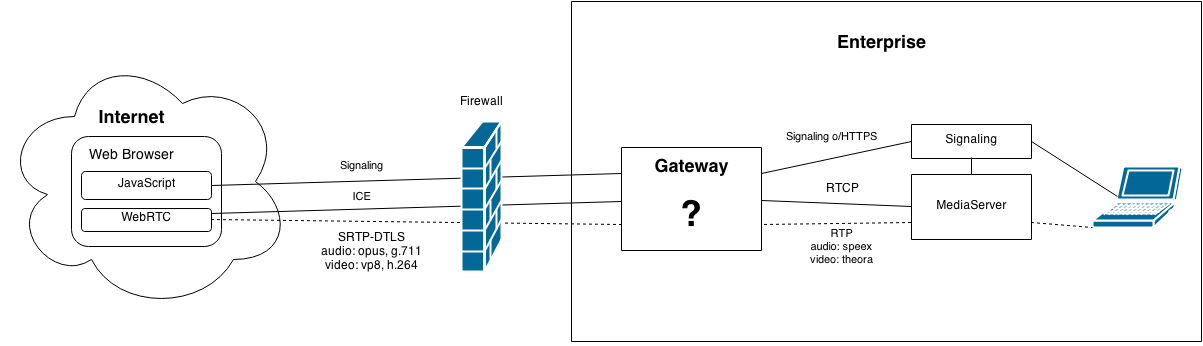
\includegraphics[scale=0.39]{gateway-unknown.png}}
\caption{WebRTC-Enterprise gateway placement}
\label{fig:gateway-layers}
\end{figure}

\subsection{The enterprise firewall}
We have to handle incoming signaling. This should not be a problem since the traffic runs over standard web protocols. Handling P2P media traffic over UDP is a different issue. In the presence of a NAT, the internal client is unaware of its public IP. It knows its internal IP, and the NAT device performs a rewriting of the source port and address in every UDP packet. A WebRTC application must first discover its public IP address to share it with a peer outside its private network. The NAT must also handle packets that arrive at the public IP, and translate to an internal destination host IP and port. If this entry doesn't exist, then the packet is simply dropped. This is a problem for mobile devices that change their IP address all the time, depending on which network they are currently connected to, since we cannot explicitly configure the internal route for every IP address. TCP connections handle this with a handshake, but with UDP there is no handshake. WebRTC solves this by using the ICE technique mentioned in section~\ref{sec:ice}.

In the \gls{wrtc} world, the media plane is designed to avoid having to relay media streams. The goal is to have pure P2P connections, but this is not going to work when communicating with peers inside an enterprise network. In the enterprise world, it is common to have full control over the media plane, and in most cases use some kind of media server. It is also common to use a \gls{sbc} to control incoming media traffic. WebRTC media flows would probably be blocked by most \gls{sbc}s, so we have to find some way of detecting and applying policy to WebRTC media flows. This is a bigger topic that I will go more deeply into in the next chapter.

\subsection{The signaling proxy}
First we have to figure out how to authenticate the users. VA uses username/password authentication or single sign-on (fully integrated with the enterprise Domain Controller using Kerberos), so we need to figure out how to do this in the browser. Secondly, we need to translate the signaling. \gls{wrtc} does not define a standard way to perform signaling, but this has to be implemented and integrated with typical enterprise authentication models. Finally, negotiating the SDP has to be handled. The SDP should be included in the messages exchanged through signaling.
 

\subsection{The transport proxy}
We have to handle incoming ICE requests from a STUN or TURN server. This is why we have to implement ICE if we want to be able to cross the NAT/firewall. Also the \gls{wrtc} specification says that support for \gls{ice} and \gls{srtp}-\gls{dtls} are mandatory. Encryption is hardly ever used in the enterprise world, so this is another challenge. If encryption is used, it is more common to use \gls{srtp}-\gls{sdes} with the keys being handled on the signaling plane, rather than in the media plane that is the case with \gls{dtls}. We also need to both decrypt and encrypt the media streams from SRTP to RTP and vice versa. \gls{wrtc} uses one-way media streams, while an enterprise system usually expects to receive bi-directional streams. WebRTC says to multiplex the streams, so we have to figure out how in this component.

\subsection{The transcoder}
We need to figure out how to do transcoding, but the biggest issue here is probably which codecs we need to implement. The \gls{ietf} has landed on two default audio codecs, but has not as of 16th of May 2014 decided on which video codec to use yet. The most typical enterprise video codec used is H.264, but right now the \gls{ietf} are deciding between both H.264 and VP8. For VA's case the Speex and Theora codecs have to be supported currently.
\\
\begin{figure}[here]
\centerline{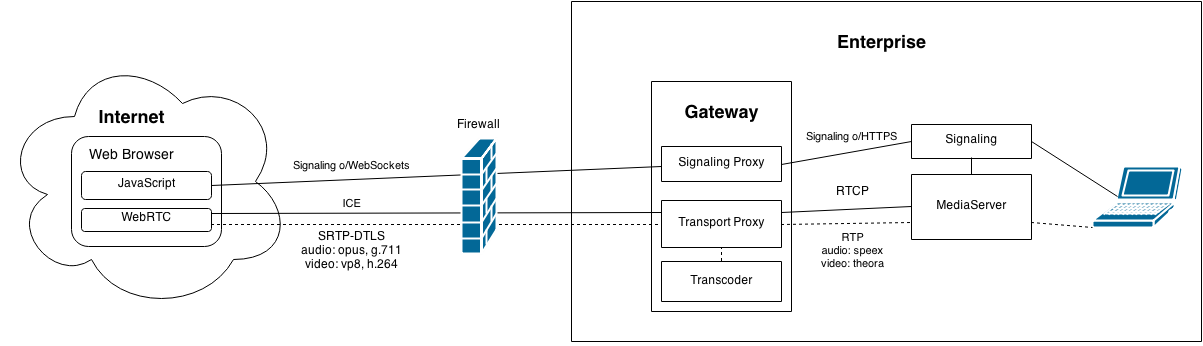
\includegraphics[scale=0.4]{gateway-suggested.png}}
\caption{WebRTC-Enterprise suggested gateway}
\label{fig:gateway}
\end{figure}

\section{Summary}
The first iteration of \gls{rtcweb} is still under development, and not all protocols and codecs to be used have been fixed yet. In theory it is possible (there are a few proprietary solutions already available) to create a gateway and it has been done before, but mostly under closed source. In Figure \ref{fig:gateway} we see the suggested gateway components. The most demanding challenges are how to handle the signaling, translation of the media, and crossing the enterprise firewall. In the next chapters I will go deeper into each component mentioned above.